\begin{abstract}
\label{sec:abstract}

{\bf Executive Summary}\\

The Transiting Exoplanet Survey Satellite (\textit{TESS}) will perform
a two-year, nearly all-sky survey for transiting exoplanets.  There do
not appear to be any fundamental obstacles to continuing science
operations for at least several years after this Primary Mission.  Any
Extended Mission will likely need to be organized while the Primary
Mission is occupying most of the TESS team's full attention.  The
purpose of this Memo, and the accompanying Wiki document, is to
provide a head start to those who are planning and proposing for an
Extended Mission.

The choice of an Extended Mission is likely to be influenced by many
factors besides the prospects for planet detection.  We have created
an editable document on the TESS wiki to raise and discuss those broad
issues.  This Memo is narrowly focused on planet detection.  We try to
anticipate the quantities and types of planets that would be detected
during several plausible scenarios for a one-year Extended Mission
following the two-year Primary Mission. We use Monte Carlo simulations
to compare different strategies for scanning the sky during one year
of operations, and try to interpret the results and their implications
for future years.  For simplicity we do not compare different choices
for the cadence of photometric measurements or in the metrics for
target selection, although different choices might prove to be
advantageous and should be studied in future work.

Throughout this report we consider six different scenarios for Year 3
of the TESS mission, illustrated in Figure~\ref{fig:strategies}:
\begin{figure*}[!b]
	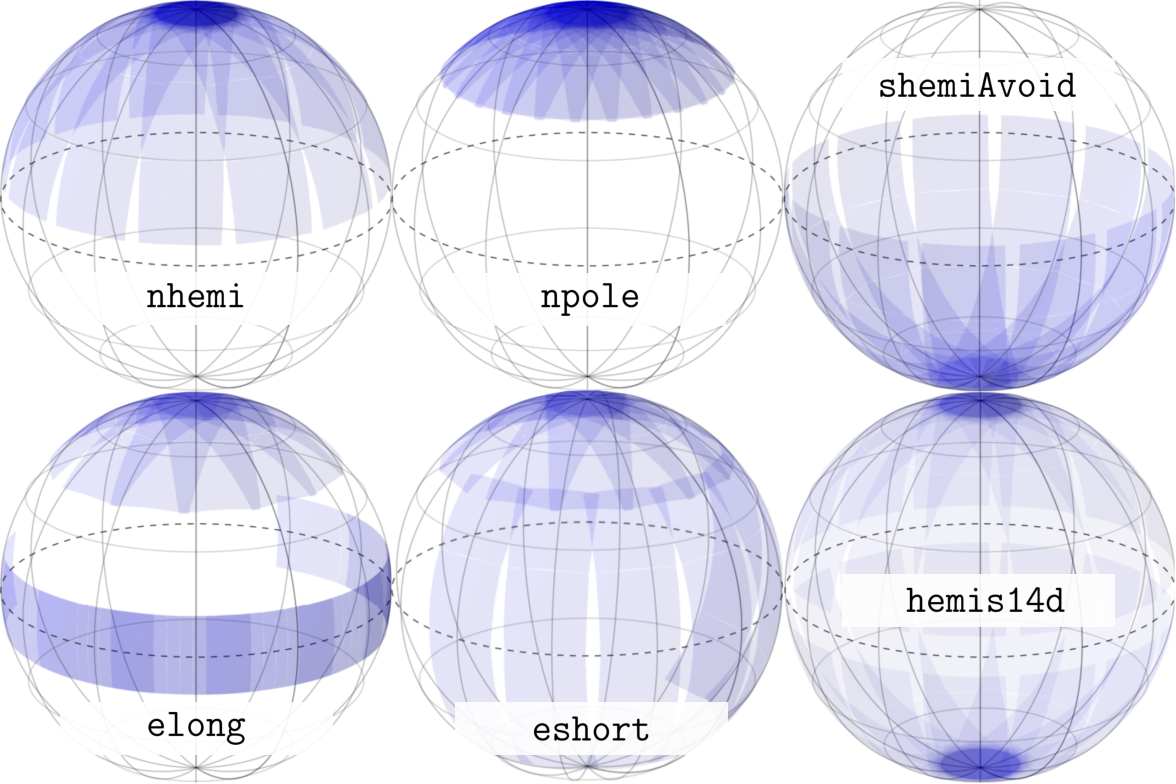
\includegraphics[width=5in]{figures/proposed_pointings_texttt.pdf}
	\caption{Six proposed pointing strategies for a \tess extended
          mission, visualized in ecliptic coordinates.  Note that none
          of these scenarios spend the entire year observing the
          ecliptic; we concluded that such a plan would be inadvisable
          because of interruptions by the Earth and Moon (see
          Fig.~\protect\ref{fig:earth_moon_elong}).}
	\label{fig:strategies}
\end{figure*}

\begin{enumerate}

\item {\it HEMI}, which re-observes one of the ecliptic hemispheres in
  essentially the same manner as in the Primary Mission (i.e.,
  neglecting the zone within $6^\circ$ of the ecliptic);
  
\item {\it HEMI+ECL}, which re-observes one of the ecliptic
  hemispheres, but this time covering the entire hemisphere at the
  expense of the continuous-viewing zone near the pole;
  
\item {\it POLE}, which focuses on one of the two ecliptic poles;

\item {\it ECL-LONG}, which has a series of pointings with the long
  axis of the field-of-view along the ecliptic (in combination with
  some fields near the ecliptic pole, when the Earth or Moon would
  prevent effective observations of the ecliptic);
  
\item {\it ECL-SHORT}, which has a series of pointings with the short
  axis of the field-of-view along the ecliptic (again in combination
  with some fields near the ecliptic pole);
  
\item {\it ALLSKY}, which covers nearly the entire sky with 14-day
  pointings (as opposed to the 28-day pointings of the Primary
  Mission), by alternating between northern and southern hemispheres.
 
\end{enumerate}

We simulate the results based on the methodology of~\citet{Sullivan_2015}, after bug fixes and enhancements by Luke Bouma in
consultation with Josh Winn. Additional inputs were provided by Jacobi
Kosiarek and Peter McCullough, as described in the text.

Some of the most important findings are:
\begin{enumerate}

\item The overall quantity of detected planets does not depend
  strongly on the sky-scanning schedule.  Among the six scenarios
  considered here, the number of newly-detected sub-Neptune planets is
  the same to within about 30\%.

\item The number of newly-detected sub-Neptune planets in Year 3 is
  approximately the same as the number detected in either Year 1 or
  Year 2.  Thus, we do not expect a sharp fall-off in the planet
  discovery rate in Year 3.  This is because the Primary Mission will
  leave behind many short-period transiting planets with bright host
  stars, with a signal-to-noise ratio just below the threshold for
  detection.  These planets can be detected by collecting more data in
  Year 3.

\item Regarding newly detected sub-Neptunes, the \hemis, \npole, and
  \shemiAvoid\ strategies offer the greatest number (1300-1400, as
  compared to the 1250 during each year of the Primary Mission).
 
\item Regarding planets with orbital periods $\gsim$20 days, the
  \hemis, \npole, and \nhemi\, strategies would discover twice as many
  such planets as will be discovered in each year of the Primary
  Mission. This would help to overcome one of the main limitations of
  the Primary Mission: the strong bias toward shorter orbital periods.

\item Regarding new planets with very bright host stars ($I_c<10$),
  the \hemis, \shemiAvoid, and \eshort\ strategies offer the greatest
  numbers ($\sim$190, about the same as are found in each year of the
  Primary Mission; see Table~\ref{tab:icmag_meta}).

\item Regarding planets with near-terrestrial insolation ($0.2 <
  S/S_\odot < 2$), all the strategies considered here offer similar
  numbers (about 120, as compared to 105 in each year of the Primary
  Mission).
    
\item Apart from detecting new planets, a potentially important
  function of an Extended Mission would be to improve our ability to
  predict the times of future transits and eclipses of TESS-detected
  planets.  With data from the Primary Mission alone, the uncertainty
  in transit ephemerides will inhibit follow-up observations after
  only a few years.
  
\end{enumerate}

The rest of this report is organized as follows.
Sec.~\ref{sec:approach} discusses how we selected and compared different pointing strategies, as well as how we modeled \tesss observations and planet detections.
Sec.~\ref{sec:input_assumptions} gives a list of the most important assumptions we made for the simulations.
Sec.~\ref{sec:newly_detected_planet_metrics} compares the simulated populations of newly-detected planets, for the 6 different scenarios under consideration.
Sec.~\ref{sec:gtr_1yr_horizon}) discusses some considerations and implications for future years of the Extended Mission, beyond the one-year scenarios that were simulated
in detail.
Sec.~\ref{sec:ephemeris_times}) discusses the critical issue of the uncertainty in transit ephemerides.
Sec.~\ref{sec:risks_caveats} discusses the reliability and limitations of our methodology.
Sec.~\ref{sec:conclusions} presents our conclusions, and recommends avenues for further study.

\end{abstract}
